% Manual for Tali Forth for the 65c02
% Scot W. Stevenson <scot.stevenson@gmail.com>
% First version: 02. Mar 2018
% This version: 20. May 2018
% See:
% - https://en.wikibooks.org/wiki/LaTeX/Document_Structure#Document_classes
% - https://www.sharelatex.com/blog/2013/08/02/thesis-series-pt1.html
% Install additional fonds with "sudo apt-get install texlive-fonts-extra"
% https://launchpad.net/ubuntu/xenial/+package/texlive-fonts-extra
\documentclass[a4paper,notitlepage]{report}
\usepackage[width=150mm,top=25mm,bottom=25mm]{geometry}
\usepackage{fancyhdr}
\pagestyle{fancy}

\usepackage{graphicx}
\usepackage{makeidx}
\makeindex

\usepackage{sourcecodepro}      % for monospaced

\usepackage{listings}
\lstset{basicstyle=\ttfamily,breaklines=true} % use monospace

\usepackage{color}
\usepackage[colorlinks=true]{hyperref}   % must be last

% Add real titlepage

\title{The Tali Forth 2 Manual (ALPHA)}
\author{Scot W.~Stevenson}
\date{\today}


% --------------------------------
\begin{document}

\maketitle

\begin{abstract}
        Tali Forth 2 is a bare-metal ANSI(ish) Forth for the 65c02 8-bit MPU. 
        It aims to be, roughly in order of importance: 

        \begin{description}

        \item [Easy to try.]
                \href{https://github.com/scotws/TaliForth2}{Download the source}
                -- or even just the binary -- and you can immediately
                run it in an emulater. This lets you experiment with a
                working 8-bit Forth for the 65c02 without any special
                configuration.

        \item [Simple.] The subroutine-threaded (STC) design and happily
                overcommented source code give hobbyists the chance to study a
                working Forth at the lowest level. The manual -- this
                document -- explains structure and code in detail. The aim
                is to make it easy to port Tali Forth 2
                to various 65c02 hardware projects.

        \item [Specific.] Many Forths available are `general' implementations with
                a small core adapted to the target processor. Tali Forth 2 was
                written as a "bare metal Forth" for the 65c02 8-bit MPU
                and that MPU only, with its strengths and limitations in
                mind.

        \item [Standardized.] Most Forths available for the 65c02 are based on ancient,
                outdated templates such as FIG Forth. Learning Forth with them is like
                trying to learn modern English by reading Chaucer. Tali
                Forth (mostly) follows the current ANSI Standard.
\end{description}

        Tali Forth is hosted at GitHub at
        \href{https://github.com/scotws/TaliForth2}{https://github.com/scotws/TaliForth2}. 
        The discussion thread is at 6502.org at
        \href{http://forum.6502.org/viewtopic.php?f=9\&t=2926}{http://forum.6502.org/viewtopic.php?f=9\&t=2926}.
        
\end{abstract}

% --------------------------------
\tableofcontents
\listoffigures
\listoftables

% --------------------------------
\part{Introduction}

\chapter{Why}
        % The Why of Tali Forth
% Scot W. Stevenson

\section{The big picture}

This section provides background information on Forth, the 6502 processor, and
what anybody would want to combine the two. It can be safely skipped.

\subsection{The 6502 MPU}

Humanity reached the high point of processor design with the 6502\index{6502} in
1976. Created by a team including Chuck Peddle\index{Peddle, Chuck} and Bill
Mensch\index{Mensch, Bill}, it was the engine that powered the 8-bit home
computer revolution of the 1980s.\footnote{Rumor has it that there was another
MPU called `Z80'\index{Z80} at the same time, but it ended up being a mere
footnote.} The VIC-20\index{VIC-20}, Commodore PET\index{Commodore PET}, Apple
II\index{Apple II}, and Atari 800\index{Atari 800} all used the 6502, among
others. 

\begin{figure}[h !]
        \centering
        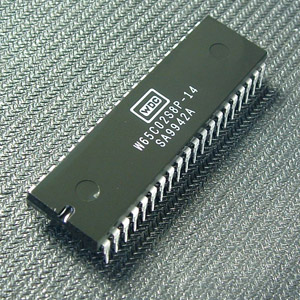
\includegraphics[width=0.5\textwidth]{pics/W65c02}
        \caption{\textit{The 65c02 MPU.} Photographer: Anthony King, released in 
        the public domain}
        \label{fig:65c02}
\end{figure}

More than 40 years later, the processor is still in production by the \href
{http://www.westerndesigncenter.com/wdc/w65c02s-chip.cfm} {Western Design
Center}\index{WDC}. Apart for commercial uses, there is an active hobbyist scene
centered on the website \href{http://6502.org/}{6502.org}.\index{6502.org} Quite
a number of people have built their own 8-bit computers based on this chip. 

The most important variant produced today is the \href
{https://en.wikipedia.org/wiki/WDC\_65C02}{65c02}\index{65c02}, a CMOS chip with
some additional instructions. Tali Forth 2 is specifically designed for this
chip and this chip only.

Why program in 8-bit assembler? The 65c02 is fun to work with because of its
clean instruction set architecture (ISA)\index{instruction
set!architecture}\index{ISA|see {instruction set}}. 


\subsection{Forth}

\begin{quote}
        But Forth is also like a high-wire act; if C gives you enough rope to
        hang yourself, Forth is a flamethrower crawling with cobras.
\end{quote}
\begin{flushright}
        -- Elliot Williams,\index{Williams, Elliot} \href{https://hackaday.com/2017/01/27/forth-the-hackers-language/}{
        \textit{Forth: The Hacker's Language}}
\end{flushright}

Forth\index{Forth|textbf} is black sheep among the program languages. Invented
by Chuck Moore\index{Moore, Chuck} in the 1960s for work with radio astronomy,
it is stack-based, uses reverse polish notation (RPN)\index{RPN|see {reverse
polish notation}}\index{reverse polish notation} and a threaded interpreter
model. 

(HIER HIER)

There is no way this document can support an introduction to Forth. There are
quite a number only, such as \textit{A Beginner's Guide to Forth} by
J.V.~Nobel\cite{nobel} or the classic (but slightly dated) \textit{Thinking in
Forth}\cite{brodie03} by Leo Brodie\index{Brodie, Leo}.  Gforth\index{Gforth}
comes with its own
\href{http://www.complang.tuwien.ac.at/forth/gforth/Docs-html/Tutorial.html}{tutorial}.

Once you have grasped the basic of the language, do yourself a favor and read
\textit{Thinking in Forth} by Brodie\cite{brodie84}\index{Brodie, Leo}. 


\section{Writing your own Forth}


\chapter{Overview of Tali Forth}
        % Overview of Tali Forth
% Scot W. Stevenson

% -------------------------------------
\section{Design considerations}

\subsection{Types of Forth}

\subsubsection{ANSI Forth}\index{ANSI Forth|textbf}

FIG Forth\index{FIG Forth|textbf}


\subsubsection{Threadding model}


\subsubsection{Cell size}\index{cell!size}



% -------------------------------------
\section{Design decisions}

\subsection{Where to put the TOS}

\subsection{Implementation of the Data Stack}


% --------------------------------
\part{User Guide}

\chapter{Installing}
        \section{Downloading}

Tali Forth was created to be easy to get started with. In fact, all you should
need is the \texttt{ophis.bin} binary file and the
\texttt{py65mon}\index{py65mon@\texttt{py65mon}} simulator.

\subsection{Downloading Tali Forth}

The newest version of Tali Forth 2 lives on GitHub\index{GitHub} at
\href{https://github.com/scotws/TaliForth2}{https://github.com/scotws/TaliForth2}.
You can either clone the code with \texttt{git}\index{git@\texttt{git}} or
simply download it. To just try the program, all you need is the
\texttt{ophis.bin} binary. 

\subsection{Downloading the py65mon Simulator}\index{py65mon|textbf}

Tali was written to run out of the box on the 
\texttt{py65mon} simulator from
\href{https://github.com/mnaberez/py65}{https://github.com/mnaberez/py65}. This
is a Python\index{Python} program that should run on various operating systems. 

To install py65mon on Linux\index{Linux}, use the command \texttt{sudo pip
install -U py65}. If you don't have PIP\index{PIP} installed, you will have to
add it first with \texttt{sudo apt-get install python-pip}.  There is a
\texttt{setup.py} script as part of the package.

\section{Running the binary}

To start the emulator, run:
\begin{lstlisting}[frame=lines]
        py65mon -m 65c02 -r ophis.bin
\end{lstlisting}

\noindent Note that the option \texttt{-m 65c02} is required, because Tali Forth
makes extensive use of the additional commands of the CMOS version and will not
run on a stock 6502 MPU.



\chapter{Running}
        % Chapter Running Tali Forth
% Scot W. Stevenson

\begin{quote}
	One doesn't write programs in Forth. Forth is the program.
\end{quote}
\begin{flushright}
        -- Charles Moore,\index{Moore, Charles} \textit{Masterminds of Programming}\cite{biancuzzi09}
\end{flushright}


% -------------------------------------------------
\section{Booting}\texttt{booting}

Out of the box, Tali Forth boots a minimal kernel\texttt{kernel}\index{kernel}
to connect to the py65mon\index{py65mon} simulator. By default, this stage ends
with a line such as

\begin{lstlisting}[frame=lines]
        Tali Forth 2 default kernel for py65mon (18. Feb 2018)
\end{lstlisting}

\noindent Tali Forth itself boots next, and after setting up various internal
things, compiles the high level words. This causes a slight delay, depending on
the number and length of these words. As the last step, Forth should spit out a
boot string, something to the effect of

\begin{lstlisting}[frame=lines]
        Tali Forth 2 for the 65c02
        Version ALPHA 07. Mar 2018 
        Copyright 2014-2018 Scot W. Stevenson
        Tali Forth 2 comes with absolutely NO WARRANTY
        Type 'bye' to exit
\end{lstlisting}

\noindent This functions as a primitive self-test. If you have modified the high
level Forth words\index{Forth words} in either \texttt{forth\_words.fs} or
\texttt{user\_words.fs}, the boot process might fail with a variant of the error
message `unknown word'. The built-in, native words should still work.


% -------------------------------------------------
\section{Available words}

Tali Forth comes with the following Forth words\index{Forth words} out of the
box:

\begin{lstlisting}[frame=lines]
        see within to d.r d. ud.r ud. .r u.r */mod */ mod /mod /
        action-of is defer@ defer! while until repeat else then
        if .( ( drop dup swap ! @ over >r r> r@ nip rot -rot tuck
        , c@ c! +! execute emit type . u. ? false true space 0 1
        2 2dup ?dup + - abs dabs and or xor rshift lshift pick char
        [char] char+ chars cells cell+ here 1- 1+ 2* = <> < > 0=
        0<> 0> 0< min max 2drop 2swap 2over 2variable 2r@ 2r> 2>r
        invert negate dnegate c, bounds spaces bl -trailing /string
        refill accept unused depth key allot create does> variable
        constant value s>d d>s d- d+ erase blank fill find-name '
        ['] name>int int>name name>string >body defer latestxt
        latestnt parse-name parse source source-id : ; compile, [ ]
        0branch branch literal sliteral ." s" postpone immediate
        compile-only never-native always-native nc-limit abort
        abort" do ?do i j loop +loop exit unloop leave recurse quit
        begin again state evaluate base digit? number >number hex
        decimal count m* um* * um/mod ud/mod sm/rem fm/mod \ move
        cmove> cmove pad >in <# # #s #> hold sign output input cr
        page at-xy marker words wordsize aligned align bell dump .s
        find word cold bye
\end{lstlisting}

\noindent (Call \texttt{words}\index{words@\texttt{words}} in Tali Forth for the
current list.)

Though the list might look unsorted, it actually reflects the priority in the
dictionary\index{dictionary}, that is, which words are found first. For
instance, the native words\index{native words} -- those coded in assembler --
start with \texttt{drop}\index{drop@\texttt{drop}}
\texttt{bye}\index{bye@\texttt{bye}}, which is the last word that Tali Forth
will find.\footnote{If you're going to quit, speed can't be that important} The
words before \texttt{drop} are those that are defined in high-level Forth. For
more information on the words, use the \texttt{see}\index{see@\texttt{see}}
command.

Note that the built-in words are lower case\index{case!lower}. Newly defined
words can be in any case and will be distinct -- `KASUMI' is a different word
than `Kasumi'.\index{Goto, Kasumi}


\subsection{Standards}

Tali Forth is orientated on ANSI Forth, but (currently) doesn't contain the
complete set of even the core words. Tali also adopted some words from
Gforth\index{Gforth} such as \texttt{bounds}\index{bounds@\texttt{bounds}}. In
practical terms, Tali aims to be a subset of Gforth: If a program runs on Tali,
it should run on Gforth the same way or have a very good reason not to. 

In addition, there are a few words that are specific to Gforth such as 
\texttt{nc-limit}\index{nc-limit@\texttt{nc-limit}}. 

% -------------------------------------------------
\section{Native compiling}\index{compiling!native}

As the name says, subroutine threaded code\index{threading} encodes the words as
a series of subroutine jumps. Because of the overhead caused by these jumps,
this can make the code slow. Therefore, Tali Forth enables `native compiling',
where the machine code from the word itself is included instead of a subroutine
jump. 

The parameter \texttt{nc-limit}\index{nc-limit@\texttt{nc-limit}} sets the limit
of how small words have to be to be natively compiled. To get the current value
(usually 20), check the value of the system variable: 

\begin{lstlisting}[frame=lines]
        nc-limit ?
\end{lstlisting}

\noindent To set a new limit, save the maximal allowed number of bytes in the
machine code like any other Forth variable:

\begin{lstlisting}[frame=lines]
        40 nc-limit !
\end{lstlisting}

To complete turn off native compiling, set this value to zero.


% -------------------------------------------------
\section{Underflow detection}\index{underflow!detection}

When a word tries to access more words on the stack than it is holding, an
`underflow' error occurs. Whereas Tali Forth 1\index{Tali Forth 1} didn't check
for these errors, this version does. 

However, this slows the program down. Because of this, the user can turn off
underflow detection for words that are natively compiled into new words. To do
this, set the system variable
\texttt{uf-strip}\index{uf-strip@\texttt{uf-strip}} to
\texttt{true}\index{true@\texttt{true}}. Note this does not turn off underflow
detection in the built-in words. Also, words with underflow detection which are
not included in new words through native compiling will also retain their tests.


% -------------------------------------
\section{Restarting}

Tali Forth has a non-standard word \texttt{cold}\index{cold@\texttt{cold}} that
resets the system. Note that this doesn't erase any data in memory, but just
moves the pointers back. When in doubt, you might be better off quitting and
restarting completely.


% -------------------------------------
\section{Gotchas}

Tali has a 16-bit cell size (use \texttt{1 cells 8 \* .} to get the cells size in
bits with any Forth), which can trip up calculations when compared to the
\textit{de facto} standard Gforth\index{Gforth} with 64 bits. Take this example:

\begin{lstlisting}[frame=lines]
( Gforth )      decimal 1000 100 um* hex swap u. u.  186a0 0  ok
( Tali Forth)   decimal 1000 100 um* hex swap u. u.  86a0 1  ok
\end{lstlisting}

\noindent Tali has to use the upper cell of a double-celled\index{double cell}
number to correctly report the result, while Gforth doesn't. If the conversion
from double to single is only via a \texttt{drop} instruction, this will produce
different results.


% -------------------------------------

\section{Reporting a problem}\index{feedback|textbf}\index{bugs}

The best way to point out a bug or make any other form of a comment is on Tali
Forth's page on GitHub\index{GitHub} at
\href{https://github.com/scotws/TaliForth2}{https://github.com/scotws/TaliForth2}.
There, you can `open an issue', which allows other people who might have the
same problem to help even when the author is not available.





\chapter{The Editor}
\textit{(Currently, there is no editor installed.)}


% --------------------------------
\part{Developer Guide}

\chapter{How Tali Forth works}
        
% ---------------------------------------
\section{Stack}

Tali Forth 2 uses the lowest part of the top half of Zero Page for the Data
Stack (DS). This leaves the lower half of the Zero Page for any kernel stuff the
user might require. The DS therefore grows towards the initial user variables,
see definitions.asm for details. 

> Because of the danger of underflow, it is recommended that the user kernel's
> variables are keep closer to $0100 than to $007f.

The X register is used as the Data Stack Pointer (DSP). It points to the least
significant byte of the current top element of the stack ("Top of the Stack",
TOS). 

> In the first versions of Tali, the DSP pointed to the next _free_ element of
> the stack. The new system makes detecting underflow easier and parallels the
> structure of Liara Forth. 

Initially, the DSP points to $78, not $7F as might be expected. This provides a
few bytes as a "floodplain" in case of underflow. The initial value of the DSP
is defined `dsp0` in the code in definitions.asm. 

**Single cell values:** Since the cell size is 16 bits, each stack entry
consists of two bytes. They are stored little endian (least significant byte
first). Therefore, the DSP points to the LSB of the current TOS (try reading
that last sentence to a friend who isn't into computers. Aren't abbreviations 
fun?)

Because the DSP points to the current top of the stack, the byte it points to
after boot - `dsp0` - will never be accessed: The DSP is decremented first with
two `dex` instructions, and then the new value is placed on the stack. This
means that the initial byte is garbage and can be considered part of the floodplain. 
```
               +--------------+           
               |          ... |  
               +-            -+ 
               |              |   ...
               +-  (empty)   -+
               |              |  FE,X
               +-            -+ 
         ...   |              |  FF,X
               +==============+  
        $0076  |           LSB|  00,X   <-- DSP (X Register)
               +-    TOS     -+ 
        $0077  |           MSB|  01,X
               +==============+ 
        $0078  |  (garbage)   |  02,X   <-- DSP0 
               +--------------+           
        $0079  |              |  03,X
               + (floodplain) + 
        $007A  |              |  04,X
               +--------------+           
```
_Snapshot of the Data Stack with one entry as Top of the Stack (TOS). The DSP
has been increased by one and the value written._

Note that the 65c02 system stack - used as the Return Stack (RS) by Tali -
pushes the MSB on first and then the LSB (preserving little endian), so the
basic structure is the same for both stacks. 

Because of this stack design, the second entry ("next on stack", NOS) starts at
`02,X` and the third entry ("third on stack", 3OS) at `04,X`. 

**Underflow detection** In contrast to Tali Forth 1, this version contains
underflow detection for most words. It does this by comparing the Data Stack
Pointer (X) to values that it must be smaller than (because the stack grows
towards 0000). For instance, to make sure we have one element on the stack, we
write

```
                cpx #dsp0-1
                bmi okay

                lda #11         ; error string for underflow
                jmp error
okay:
                (...)
```
For the most common cases, we have:
```
           1 cell       dsp0-1
           2 cells      dsp0-3
           3 cells      dsp0-5
```
Though underflow detection slows the code down slighly, it adds enormously to
the stability of the program.

**Double cell values:** The double cell is stored on top of the single cell.
Note this places the sign bit at the beginning of the byte below the DSP.
```
               +---------------+
               |               |  
               +===============+  
               |            LSB|  $0,x   <-- DSP (X Register) 
               +-+  Top Cell  -+         
               |S|          MSB|  $1,x
               +-+-------------+ 
               |            LSB|  $2,x
               +- Bottom Cell -+         
               |            MSB|  $3,x   
               +===============+ 
```

**Under- and overflow.** For speed reasons, Tali only checks for underflow after
the execution of a word as part of the `quit` loop. There is no checking for
overflow, which in normal operation is too rare to justify the computing expense. 

% ---------------------------------------
\section{Dictionary}


Tali Forth 2 follows the traditional model of a Forth dictionary - a linked list
of words terminated with a zero pointer. The headers and code are kept separate
to allow various tricks in the code.


## Elements of the Header

Each header is at least eight bytes long.

              8 bit     8 bit
               LSB       MSB
 nt_word ->  +--------+--------+
          +0 | Length | Status |
             +--------+--------+
          +2 | Next Header     | nt_next_word
             +-----------------+
          +4 | Start of Code   | xt_word 
             +-----------------+
          +6 | End of Code     | z_word
             +--------+--------+
          +8 | Name   |        |
             +--------+--------+
             |        |        |
             +--------+--------+
             |        |  ...   |
          +n +--------+--------+


Each word has a *name token* (nt, ``nt_word`` in the code) that points to the
first byte of the header. This is the length of the word's name string, which is
limited to 255 characters. 

The second byte in the header (index 1) is the *status byte*. It is created by
the flags defined in the file ``definitions.asm``: 

        CO - Compile Only
        IM - Immediate Word
        NN - Never Native Compile 
        AN - Always Native Compile (may not be called by JSR)

Note there are currently four bits unused. The status byte is followed by the
*pointer to the next header* in the linked list, which makes it the named token of
the next word. A ``0000`` in this position signales the end of the linked list,
which by convention is the word ``bye``. 

This is followed by the current word's *execution token* (xt, ``xt_word``) that
points to the start of the actual code. Some words that have the same
functionality point to the same code block. The *end of the code* is referenced
through the next pointer (``z_word``) to enable native compilation of the word
if allowed. 

The *name string* starts at the eighth byte. The string is _not_
zero-terminated. By default, the strings of Tali Forth 2 are lower case, but
case is respected for words the user defines, so ``quarian`` is a different
words than ``QUARIAN``. 


## Structure of the Header List 

Tali Forth 2 distinguishes between three different list sources: The *native
words* that are hard-coded in the file ``native_words.asm``, the *forth words*
which are defined as high-level words and then generated at run-time when Tali
Forth starts up, and *user words* in the file ``user_words.asm`` which is empty
when Tali Forth ships. 

Tali has an unusually high number of native words in an attempt to make the
Forth as fast as possible on the 65c02. The first word in the list - the one
that is checked first - is always ``drop``, the last one - the one checked for
last - is always ``bye``. The words which are (or are assumed to be) used more
than others come first. Since humans are slow, words that are used more
interactively like ``words`` come later. 

The list of Forth words ends with the intro string. This functions as a
primitive form of a self-test: If you see the string and only the string, the
compilation of the Forth words worked.


% ---------------------------------------
\section{Memory Map}


Tali Forth 2 was developed with a simple 32 KiB RAM, 32 KiB ROM design. 


The following drawing is not only ugly, but also not drawn to scale.


    $0000  +-------------------+  ram_start, zpage, user0
           |  User varliables  |
           +-------------------+  
           |                   |
           |  ^  Data Stack    |  <-- dsp
           |  |                |
    $0078  +-------------------+  dsp0, stack
           |                   |
           |   (Reserved for   |
           |      kernel)      |
           |                   |
    $0100  +===================+  
           |                   |
           |  ^  Return Stack  |  <-- rsp 
           |  |                |
    $0200  +-------------------+  rsp0, buffer, buffer0
           |  |                |
           |  v  Input Buffer  |
           |                   |
    $0300  +-------------------+  cp0
           |  |                |
           |  v  Dictionary    |
           |       (RAM)       |
           |                   |
           ~~~~~~~~~~~~~~~~~~~~~  <-- cp
           |                   |
           |                   |
           |                   |
    $7fff  #####################  ram_end
    $8000  |                   |  forth, code0
           |                   |
           |                   |
           |    Tali Forth     |
           |     (24 KiB)      |
           |                   |
           |                   |
    $e000  +-------------------+
           |                   |  kernel_putc, kernel_getc   
           |      Kernel       |
           |                   |
    $f000  +-------------------+  
           |   I/O addresses   |
           +-------------------+     
           |                   |
           |      Kernel       |
           |                   |
    $fffa  +-------------------+     
           |  65c02 vectors    |
    $ffff  +-------------------+     




% ---------------------------------------
\section{Input}



Tali Forth 2, like Liara Forth, follows the ANSI input model with
`refill` instead of older forms. 

There are up to four possible input sources in Forth (see C&D p. 155):

1. The keyboard ("user input device")

2. A character string in memory

3. A block file

4. A text file

To check which one is being used, we first call BLK, which gives us the number
of a mass storage block being used, or 0 for the "user input device" (keyboard).
In the second case, we use SOURCE-ID to find out where input is coming from: 0
for the keyboard, -1 (0ffff) for a string in memory, and a number n for a
file-id.

Since Tali currently doesn't support blocks, we can skip the BLK instruction and
go right to `source-id`. 


## Starting up

The intial commands after reboot flow into each other: `cold` to `abort` to
`quit`. This is the same as with pre-ANSI Forths. However, `quit` now calls
`refill` to get the input. `refill` does different things based on which of the
four input sources (see above) is active: 

1. **Keyboard entry.** This is the default. Get line of input via `accept` and
   return a TRUE flag even if the input string was empty.

2. **EVALUTE string.** Return a FALSE flag.

3. **Input from a buffer.** Not implemented at this time.

4. **Input from a file.** Not implemented at this time.


## The Command Line Interface

Tali Forth accepts input lines of up to 256 characters.

**(THE FOLLOWING PART OF THIS SECTION IS UNDER HEAVY REVIEW)**

The address of the current input buffer is stored in `cib` and is either 
`ibuffer1` or `ibuffer2`, each of which is 256 bytes long. The length of the
current buffer is stored in `ciblen` - this is the address that >IN returns. 

When a new line is entered, the address in `cib` is swapped, and the contents of
`ciblen` are moved to `piblen` (for "previous input buffer"). `ciblen` is set to
zero. 

When the previous entry is requested, the address in `cib` is swapped back, and 
`ciblen` and `piblen` are swapped as well.

SOURCE by default returns `cib` and `ciblen` as the address and length of the
input buffer. 

(http://forth.sourceforge.net/standard/dpans/a0006.htm)
(http://forth.sourceforge.net/standard/dpans/dpansa6.htm#A.6.1.2216)

At some point, this system might be expanded to a real history list.


### SAVE-INPUT and RESTORE-INPUT

(see http://forth.sourceforge.net/standard/dpans/dpansa6.htm#A.6.2.2182)



### EVALUATE

(Automatically calls SAVE-INPUT and RESTORE-INPUT)
(http://forth.sourceforge.net/standard/dpans/a0006.htm)


### STATE 

(http://forth.sourceforge.net/standard/dpans/dpans6.htm#6.1.2250)

## Literature

[C&D] Conklin, Edward K.; Rather, Elizabeth D. *Forth Programmers Handbook,*
3.rd edition


% ---------------------------------------
\section{Create/Does}

CREATE/DOES> is the most complex, but also most powerful part of Forth.
Understanding how it works in Tali Forth is important if you want to be able to
modify the code. In this text, we walk through the generation process for
a Subroutine Threaded Code (STC) such as Tali Forth. For a more general take,
see Brad Rodriguez' series of articles
http://www.bradrodriguez.com/papers/moving3.htm . There is a discussion of this
walkthrough at http://forum.6502.org/viewtopic.php?f=9&t=3153 . 

We start with the following standard example, the Forth version of CONSTANT: 

        : CONSTANT CREATE , DOES> @ ; 

We examine this in three phases or "sequences", based on Derick and Baker (see
Rodriguez for details):   


SEQUENCE I: Compiling the word CONSTANT 

CONSTANT is a "defining word", one that makes new words. In pseudocode, and
ignoring any compilation to native 65c02 assembler, the above compiles to: 

        [Header "CONSTANT"] 
        jsr CREATE
        jsr COMMA
        jsr (DOES>)         ; from DOES>
   a:   jsr DODOES          ; from DOES>
   b:   jsr FETCH
        rts

To make things easier to explain later, we've added the labels "a" and "b" in
the listing. Note that DOES> is an immediate word that adds not one, but two
subroutine jumps, one to (DOES>) and one to DODOES, which is a pre-defined
system routine like DOVAR. We'll get to it later.

(As an aside: In Tali Forth, a number of words such as DEFER are
"hand-compiled", that is, instead of using Forth such (in this case, : DEFER
CREATE ['] ABORT , DOES> @ EXECUTE ; ) we write an opimized assembler version
ourselves (see actual DEFER code). In these cases, we need to use (DOES>) and
DODOES instead of DOES> also.)


SEQUENCE II: Executing the word CONSTANT / creating LIFE 

Now when we execute

        42 CONSTANT LIFE

this pushes the RTS of the calling routine -- call it "main" -- to the 65c02's
stack (the Return Stack, as Forth calls it), which now looks like this:

        [1] RTS to main routine 

Without going into detail, the first two subroutine jumps of CONSTANT give us
this word: 

        [Header "LIFE"]
        jsr DOVAR               ; in CFA, from LIFE's CREATE
        4200                    ; in PFA (little-endian)

Next, we JSR to (DOES>). The address that this pushes on the Return Stack is
the instruction of CONSTANT we had labeled "a". 

        [2] RTS to CONSTANT ("a") 
        [1] RTS to main routine 

Now the tricks start. (DOES>) takes this address off the stack and uses it to
replace the DOVAR JSR target in the CFA of our freshly created LIFE word. We
now have this: 

        [Header "LIFE"]         
        jsr a                   ; in CFA, modified by (DOES>)
   c:   4200                    ; in PFA (little-endian)

Note we added a label "c". Now, when (DOES>) reaches its own RTS, it finds the
RTS to the main routine on its stack. This is Good Thing, because it aborts the
execution of the rest of CONSTANT, and we don't want to do DODOES or FETCH now.
We're back at the main routine. 


SEQUENCE III: Executing LIFE

Now we execute the word LIFE from our "main" program. In a STC Forth such as
Tali Forth, this executes a subroutine jump.

        jsr LIFE

The first thing this call does is push the return address to the main routine
on the 65c02's stack: 

        [1] RTS to main

The CFA of LIFE executes a subroutine jump to label "a" in CONSTANT. This
pushes the RTS of LIFE on the 65c02' stack:

        [2] RTS to LIFE ("c")
        [1] RTS to main

This JSR to a lands us at the subroutine jump to DODOES, so the return address
to CONSTANT gets pushed on the stack as well. We had given this instruction the
label "b". After all of this, we have three addresses on the 65c02's stack: 

        [3] RTS to CONSTANT ("b") 
        [2] RTS to LIFE ("c") 
        [1] RTS to main

DODOES pops address "b" off the 65c02's stack and puts it in a nice safe place
on Zero Page, which we'll call "z". More on that in a moment. First, DODOES
pops the RTS to LIFE. This is "c", the address of the PFA or LIFE, where we
stored the payload of this constant. Basically, DODOES performs a DOVAR here,
and pushes "c" on the Data Stack. Now all we have left on the 65c02's stack is
the RTS to the main routine.  

        [1] RTS to main

This is where "z" comes in, the location in Zero Page where we stored address
"b" of CONSTANT. Remember, this is where CONSTANT's own PFA begins, the FETCH
command we had originally codes after DOES> in the very first definition. The
really clever part: We perform an indirect JMP -- not a JSR! -- to this
address.

        jmp (z) 

Now CONSTANT's little payload programm is executed, the subroutine jump to
FETCH. Since we just put the PFA ("c") on the Data Stack, FETCH replaces this
by 42, which is what we were aiming for all along. And since CONSTANT ends with
a RTS, we pull the last remaining address off the 65c02's stack, which is the
return address to the main routine where we started. And that's all. 


Put together, this is what we have to code: 

DOES>: Compiles a subroutine jump to (DOES>), then compiles a subroutine jump
to DODOES.

(DOES>): Pops the stack (address of subroutine jump to DODOES in CONSTANT),
increase this by one, replace the original DOVAR jump target in LIFE. 

DODOES: Pop stack (CONSTANT's PFA), increase address by one, store on Zero
Page; pop stack (LIFE's PFA), increase by one, store on Data Stack; JMP to
address we stored in Zero Page. 


Remember we have to increase the addresses by one because of the way JSR stores
the return address for RTS on the stack on the 65c02: It points to the third
byte of the JSR instruction itself, not the actual return address. This can be
annoying, because it requires a sequence like:

        inc z
        bne +
        inc z+1 
*       (...) 

Note that with most words in Tali Forth, as any STC Forth, the distinction
between PFA and CFA is meaningless or at least blurred, because we go native
anyway. It is only with words generated by CREATE/DOES> where this really makes
sense.

% ---------------------------------------
\section{Loops}



This document gives the background on how Tali Forth as a STC Forth variant
handles loops (DO/?DO/LEAVE/LOOP/+LOOP) and branches (IF/ELSE/THEN). It is
based on a discussion at http://forum.6502.org/viewtopic.php?f=9&t=3176 , see
there for more details. Another take on this subject that handles things a bit
differently is at
http://blogs.msdn.com/b/ashleyf/archive/2011/02/06/loopty-do-i-loop.aspx


BRANCHES

Branches are easiest to understand at first, so we start with them. 

For IF-THEN, we need to compile something called a "conditional forward
branch", traditionally called 0BRANCH. Then, at run-time, if the value on the
Data Stack is false (flag is zero), the branch is taken ("branch on zero",
therefore the name). Execpt that we don't have the target of that branch yet --
it will later be added by THEN. For this to work, we remember the address after
the 0BRANCH instruction during the compilation of IF. This is put on the Data
Stack, so that THEN knows where to compile it's address in the second step.
Until then, a dummy value is compiled after 0BRANCH to reserve the space we
need. 

In Forth, this can be realized by

: IF  POSTPONE 0BRANCH HERE 0 , ; IMMEDIATE

and 

: THEN  HERE SWAP ! ; IMMEDIATE

though Tali Forth uses as much assembler as possible. Note THEN doesn't
actually compile anything at the location in memory where it is at. It's job is
simply to help IF out of the mess it created. 

If we have an ELSE, we have to add an unconditional BRANCH and manipulate the
address that IF left on the Data Stack. The Forth for this is: 

: ELSE  POSTPONE BRANCH HERE 0 , HERE ROT ! ; IMMEDIATE

THEN has no idea what has just happened, and just like before compiles its
address where the value on the top of the Data Stack told it to -- except that
this value now comes from ELSE, not IF. 



LOOPS 

Loops are far more complicated, because we have DO ?DO LOOP +LOOP UNLOOP and
LEAVE to take care of. These can call up to three addresses: One for the normal
looping action (LOOP/+LOOP), one to skip over the loop at the beginning (?DO)
and one to skip out of the loop (LEAVE). 

Based on a suggestion by Garth Wilson, we begin each loop in run-time by saving
the address after the whole loop construct to the Return Stack. That way, LEAVE
and ?DO know where to jump to when called, and we don't interfere with any
IF/THEN structures. On top of that address, we place the limit and start values
for the loop. 

The key to staying sane while designing these constructs is to first make
a list of what we want to happen at compile-time and what at run-time. Let's
start with a simple DO/LOOP.


DO AT COMPILE-TIME: 
- Remember current address (in other words, HERE) on the Return Stack (!) so 
  we can later compile the code for the post-loop address to the Return Stack
- Compile some dummy values to reserve the space for said code
- Compile the run-time code; we'll call that fragment (DO)
- Push the current address (the new HERE) to the Data Stack so LOOP knows where 
  the loop contents begin

DO AT RUN-TIME: 
- Take limit and start off Data Stack and push them to the Return Stack

Since LOOP is just a special case of +LOOP with an index of one, we can get
away with considering them at the same time. 


LOOP AT COMPILE TIME: 
- Compile the run-time part (+LOOP)
- Consume the address that is on top of the Data Stack as the jump target for 
  normal looping and compile it
- Compile UNLOOP for when we're done with the loop, getting rid of the 
  limit/start and post-loop addresses on the Return Stack 
- Get the address on the top of the Return Stack which points to the dummy
  code compiled by DO
- At that address, compile the code that pushes the address after the list
  construct to the Return Stack at run-time

LOOP AT RUN-TIME (which is (+LOOP)) 
- Add loop step to count
- Loop again if we haven't crossed the limit, otherwise continue after loop

At one glance, we can see that the complicated stuff happens at compile-time.
This is good, because we only have to do that once for each loop. 

In Tali Forth, these routines are coded in assembler. With this setup, UNLOOP
becomes simple (six PLAs -- four for the limit/count of DO, two for the address
pushed to the stack just before it) and LEAVE even simpler (four PLAs for the
address). 




\chapter{Developing}
        % Developing Tali Forth 2

\begin{quote}
        Programming computers can be crazy-making.
\end{quote}
\begin{flushright}
        -- Leo Brodie,\index{Brodie, Leo}\textit{Thinking Forth}\cite{brodie84}
\end{flushright}



\section{Adding new words}

The easiest way to add new words to Tali Forth is to include them in the file
\texttt{forth\_code/user\_words.fs}. 


\section{Deeper changes}

Tali Forth was not only placed in the public domain to honor the tradition of
giving the code away freely. It is also to let people play around with it and
adapt it to their own machines. This is also the reason it is (perversely)
overcommented.

To work on the internals of Tali Forth, you will need the Ophis\index{Ophis
assembler|textbf} assembler.

\subsection{The Ophis Assembler}

Michael Martin's\index{Martin, Michael} Ophis Cross-Assember can be downloaded from
\href{http://michaelcmartin.github.io/Ophis/}{http://michaelcmartin.github.io/Ophis/}.
It uses a slightly different format than other assemblers, but is in
Python\index{Python} and
therefore will run on almost any operating system. To install Ophis on Windows,
use the link provided above. For Linux\index{Linux}:

\begin{lstlisting}[frame=lines]
        git clone https://github.com/michaelcmartin/Ophis
        cd Ophis/src
        sudo python setup.py install
\end{lstlisting}

Switch to the folder where the Tali code lives, and run the Makefile with a
simple \texttt{make} command. This also updates the file listings in the
\texttt{docs} folder. 

Ophis has some quirks. For instance, you cannot use math symbols in label names,
because it will try to perform those operations. Use underscores for label names
instead.

\subsection{General notes}

\begin{itemize}

        \item The X register\index{X register} should not be changed without
                saving its pointer status.

        \item The Y register\index{Y register} is free to be changed by
                subroutines. This means it should not be expected to survive
                subroutines unchanged.

        \item All words should have one point of entry -- the \texttt{xt\_word}
                link -- and one point of exit at \texttt{z\_word}. In may cases,
                this means a branch to an internal label \texttt{done} right
                before \texttt{z\_word}.

        \item Because of the way native compiling works, the usual trick of
                combining \texttt{jsr/rts} pairs to a single \texttt{jmp}
                (usually) doesn't work.

\end{itemize}


\subsection{Coding style}\index{style, coding}

Until I get around to writing a tool for Ophis\index{Ophis assembler} assembler
code that formats the source file the way gofmt does for Go\index{Go} (golang),
I work with the following rules:

\begin{itemize}

        \item Actual opcodes are indented by \textbf{two tabs}

        \item Tabs are \textbf{eight characters long} and converted to spaces

        \item Function-like routines are followed by a one-tab indented
                `function doc' based on the Python 3\index{Python} model: Three
                quotation marks at the start, three at the end it its own line,
                unless it is a one-liner. This should make it easier to
                automatically extract the docs for them at some point.

        \item The native words have a special commentary format that allows the
                automatic generation of word list by a tool in the tools folder,
                see there for details.

        \item Assembler mnenomics are lower case. I get enough uppercase
                insanity writing German, thank you very much.

        \item Hex numbers are also lower case, such as \texttt{\$FFFE}

        \item Numbers in mnemonics are a stripped-down as possible to reduce
                visual clutter: \texttt{lda 0,x} instead of \texttt{lda \$00,x}.

        \item Comments are included like popcorn to help readers who are new
                both to Forth and 6502 assembler.

\end{itemize}


\section{Code Cheat Sheet}\index{cheat sheet, code}

\subsection{The Stack Drawing}\index{stack}
This is your friend and should probably go on your wall or something.

\begin{lstlisting}[frame=single]
                +--------------+
                |          ... |
                +-            -+
                |              |   ...
                +-  (empty)   -+
                |              |  FE,X
                +-            -+
          ...   |              |  FF,X
                +==============+
         $0076  |           LSB|  00,X   <-- DSP (X Register)
                +-    TOS     -+
         $0077  |           MSB|  01,X
                +==============+
         $0078  |  (garbage)   |  02,X   <-- DSP0
                +--------------+
         $0079  |              |  03,X
                + (floodplain) +
         $007A  |              |  04,X
                +--------------+
\end{lstlisting}

\subsection{Coding idioms}
While coding a Forth, there are certain assembler fragments that get repeated
over and over again. These could be included as macros, but that can make the
code harder to read for somebody only familiar with basic assembly.

Some of these fragments could be written in other variants, such as the `push
value' version, which could increment the DSP twice before storing a value. We
try to keep these in the same sequence (a "dialect" or "code mannerism" if you
will) so we have the option of adding code analysis tools later.

\begin{description}

        \item [\texttt{drop}] cell of top of the Data Stack 

                \begin{lstlisting}[frame=lines]
                inx
                inx
                \end{lstlisting}

        \item [\texttt{push}] a value to the Data Stack.  Remember the Data Stack
                Pointer (DSP, the X register of the 65c02) points to the LSB of
                the TOS value.

                \begin{lstlisting}[frame=lines]
                dex
                dex
                lda $<LSB>      ; or pla, jsr kernel_getc, etc.
                sta 0,x
                lda $<LSB>      ; or pla, jsr kernel_getc, etc.
                sta 1,x
                \end{lstlisting}

        \item [\texttt{pop}] a value off the Data Stack

                \begin{lstlisting}[frame=lines]
                lda 0,x
                sta $<LSB>      ; or pha, jsr kernel_putc, etc
                lda 1,x
                sta $<MSB>      ; or pha, jsr kernel_putc, etc
                inx
                inx
                \end{lstlisting}

\end{description}

\subsection{vi shortcuts}

One option for these is to add abbreviations to your favorite editor, which
should of course be vim, because vim is cool. There are examples for that
further down. They all assume that auto-indent is on and we are two tabs in with
the code, and use \texttt{\#} at the end of the abbreviation to keep them
separate from the normal words. My \texttt{\textasciitilde/.vimrc} file contains the following
lines for work on \texttt{.asm} files:
 

\begin{lstlisting}[frame=lines]
 ab drop# inx<tab><tab>; drop<cr>inx<cr><left>
 ab push# dex<tab><tab>; push<cr>dex<cr>lda $<LSB><cr>sta $00,x<cr>lda $<MSB><cr>sta $01,x<cr><up><up><up><up><end>
 ab pop# lda $00,x<tab><tab>; pop<cr>sta $<LSB><cr>lda $01,x<cr>sta $<MSB><cr>inx<cr>inx<cr><up><up><up><up><up><end>
\end{lstlisting}
 


\chapter{Future plans}
        \textit{(See the file TODO.txt)}

% --------------------------------

\appendix

\chapter{FAQ}
        \section{Why does Tali Forth take so long to start up?}

After the default kernel string is printed, you'll notice a short pause that
didn't occur with Tali Forth 1. This is because Tali Forth 2 has more words
defined in high-level Forth (see \texttt{forth-words.asm}) than Tali did. The
pause happens because they are being compiled on the fly.

\section{Why `Tali' Forth?}

I like the name, and we're probably not going to have anymore kids I can give it
to.

(If it sounds vaguely familiar, you're probably thinking of Tali'Zorah vas
Normandy, a character in the `Mass Effect' universe created by EA / BioWare.
This software has absolutely nothing to do with either the game or the companies
and neither do I, expect that I've played the games and enjoyed them, though I
do have some issues with \emph{Andromeda}. Like what happened to the quarian ark?)

\section{Then who is `Lara'?}

Liara Forth is a STC Forth for the big sibling of the 6502, the 65816. Tali 1
came first, then I wrote Liara with that knowledge and learned even more, and
now Tali 2 is such much better for the experience. Oh, and it's another `Mass
Effect' character.



\chapter{Testing Tali Forth}
        % Tests for Forth
% Scot W. Stevenson
% TODO rename examples so letters coincide with themes

Tali Forth 2 operates in a hardware environment that makes built-in
tests\index{testing|textbf} pretty much impossible. The following collection of
Forth snippets provides a basic way of testing at least some party by hand.

For stress testing, the \texttt{user\_words.fs} routines contain routines such as
a Mandelbrot\index{Mandelbrot} program that can be uncommented and run.

% ----------------------------------------
\section{The interpreter}\index{interpreter}

\subsection{\texttt{>in} tests}

From
https://www.complang.tuwien.ac.at/forth/gforth/Docs-html/The-Text-Interpreter.html

\begin{lstlisting}
        : lat ." <foo>" ;
        : flat ." <bar>" >in dup @ 3 - swap ! ; 
\end{lstlisting}

\noindent A simple \texttt{flat} should print \texttt{<bar><foo>}. A bit more complicated:

\begin{lstlisting}
        char & parse jack& type
\end{lstlisting}

\noindent This should print \texttt{jack}.


% ----------------------------------------
\section{Defining words}

\subsection{\texttt{create} and \texttt{does>}}
The simplest test is to redefine \texttt{constant}:

\begin{lstlisting}
        : aaa create , does> @ ; 
\end{lstlisting}


\subsection{\texttt{literal}}

\begin{lstlisting}
        : aaa [ 1 ] literal ;
\end{lstlisting}

\noindent This should put 1 on the Data Stack at run time.


\subsection{\texttt{bracket-tick}}

\begin{lstlisting}
        : aaa ['] words execute ;     \ should print all words known
\end{lstlisting}


\subsection{\texttt{postpone}}

\begin{lstlisting}
        : say-hello ." Hello" ; immediate
        : greet postpone say-hello ." I speak Forth" ;
\end{lstlisting}

\noindent Note that \texttt{greet} won't print \texttt{Hello} right away

\noindent Based on https://www.forth.com/starting-forth/11-forth-compiler-defining-words/


\subsection{\texttt{find-name}}

\begin{lstlisting}
        s" words" find-name name>string type
\end{lstlisting}

\noindent should print \texttt{words}


\subsection{\texttt{words} vs \texttt{parse}}

Taken from Conklin \& Rather p. 160

\begin{lstlisting}
        : test1 ( "name" -- )  32 word count type ; 
        : test2 ( "name" -- )  32 parse type ; 
\end{lstlisting}

\noindent Results of calls with `ABC' should give identical result if there are no
leading spaces. However, with leading spaces, TEST2 will find an empty string
and abort, then throw an error because ABC will not be found in the dictionary.

% ----------------------------------------
\section{Looping}

The looping constructs are the most complicated parts of Tali Forth. Currently,
we use the Return Stack instead of the more traditional Data Stack as the
mythical Forth `Control Stack'.

\subsection{Basic looping}

Test normal loop:
\begin{lstlisting}
        : aaa 11 1 do i . loop ;        
\end{lstlisting}

\noindent This should simply produce the numbers 1 to 10. Then, break up the
loop over multiple lines because it turns out this can be tricky:

\begin{lstlisting}
        : bbb 11 1 do 
          i . loop ; 
\end{lstlisting}

\noindent Following Gforth\index{Gforth}, we then should test other variants:

\begin{lstlisting}
        : bbb1 -1 0 ?do i . -1 +loop ;
\end{lstlisting}

\noindent This should produce `0 -1', while

\begin{lstlisting}
        : bbb2 0 0 ?do i . -1 +loop ;
\end{lstlisting}

\noindent should print nothing.


\subsection{Looping with \texttt{if}}

Including \texttt{if} in a loop is the ultimate test if everything is correct
with our stack machanics. First, a simple version will do:

\begin{lstlisting}
        : ccc 11 1 do i dup 5 > if . then loop ; 
\end{lstlisting}

\noindent This should produce \texttt{6 7 8 9 10}. The next step is to continue
with some instructions after the \texttt{then} -- this actually revealed a
stupid bug in the ALPHA version of Tali Forth 2.

\begin{lstlisting}
        : ccc 11 1 do i dup 2 = if ." two! " then . loop ;
\end{lstlisting}

\noindent This should print the string right before the number two.

\subsection{Nested loops}

\noindent A simple test of nested loops is found in
\href{https://www.forth.com/starting-forth/6-forth-do-loops/}{\textit{Starting
Forth}}:

\begin{lstlisting}
        : ddd cr 11 1 do
            11 1 do 
                i j * 5 u.r 
            loop cr loop ;
\end{lstlisting}

\noindent This should print a multiplication table from 1x1 to 10x10.

\subsection{\texttt{exit}}

\begin{lstlisting}
        : eee1 true if exit then ." true" ; 
        : eee2 false if exit then ."false" ; 
\end{lstlisting}

\noindent First word should just return with \texttt{ok}, second word prints \texttt{false}.


\subsection{\texttt{unloop}}

\begin{lstlisting}
        : fff 11 1 do i dup 8 = if drop unloop exit then . loop ." Done" ; 
\end{lstlisting}

\noindent should produce \texttt{1 2 3 4 5 6 7} (with no \texttt{Done})


\subsection{\texttt{leave}}

\begin{lstlisting}
        : ggg 11 1 do i dup 8 = if leave then . loop ." Done" drop ; 
\end{lstlisting}

\noindent should produce \texttt{1 2 3 4 5 6 7 Done} (note \texttt{Done} printed)

The Data Stack should be empty after all of these words, check with \texttt{.s}


\subsection{\texttt{recurse}}
\index{recursion}
\index{recurse@\texttt{recurse}}

\begin{lstlisting}
        : hhh ( a b -- gcd ) ?dup if tuck mod recurse then ;
\end{lstlisting}

\noindent Which should produce 16 for 784 48 hhh. 

% Source: 
% [http://galileo.phys.virginia.edu/classes/551.jvn.fall01/primer.htm]
% (http://galileo.phys.virginia.edu/classes/551.jvn.fall01/primer.htm)

Also, the classic (here from the ANSI Forth documentation):

\begin{lstlisting}
        : factorial ( u -- u ) 
           dup 2 < if drop 1 exit then 
           dup 1- recurse * ;
\end{lstlisting}

\noindent For 5, the result should be 120.


% ----------------------------------------

\section{Math routines}\index{math}

% TODO For examples of interger divsion, see
% [http://www.forth200x.org/documents/html/usage.html#usage:div]


\subsection{\texttt{fm/mod}}
\index{fm/mod@\texttt{fm/mod}|textbf}

\begin{lstlisting}
        : fm swap s>d rot fm/mod swap . . ; 
\end{lstlisting}

\noindent Should give you: 
% TODO convert to table
\begin{lstlisting}
        10 7 --> 3 1
        -10 7 --> 4 -2 
        10 -7 --> -4 -2
        -10 -7 --> -3 1
\end{lstlisting}


\subsection{\texttt{sm/rem}}
\index{sm/rem@\texttt{sm/rem}|textbf}

\begin{lstlisting}
        : sm swap s>d rot sm/rem swap . . ; 
\end{lstlisting}

\noindent Should give you: 
% TODO convert to table
\begin{lstlisting}
        10 7 --> 3 1
        -10 7 --> -3 -1 
        10 -7 --> 3 -1
        -10 -7 --> -3 1
\end{lstlisting}


\chapter{Thanks}
        Tali Forth would never have been possible without the help of a very large
number of people, very few of which I have actually even met.

\index{6502.org}



\begin{thebibliography}{99}

\bibitem{biancuzzi09}
        Federico \textbf{Biancuzzi},
  	\textit{Masterminds of Programming},
	O'Reilly Media
  	1st edition,
	2009.

\bibitem{brodie03}
        Leo \textbf{Brodie},
  	\textit{Starting Forth},
  	New edition 2003,
        \href{https://www.forth.com/starting-forth/}{https://www.forth.com/starting-forth/}

\bibitem{brodie84}
        Leo \textbf{Brodie},
  	\textit{Thinking in Forth},
  	1984,
        \href{http://thinking-forth.sourceforge.net/\#21CENTURY}{http://thinking-forth.sourceforge.net/\#21CENTURY}

\bibitem{leventhal79}
        Lance A. \textbf{Leventhal},
  	\textit{6502 Assembly Language Programming},
	OSBORNE/McGRAW-HILL
	1979.

\bibitem{nobel}
        J.V.~\textbf{Nobel},
  	\textit{A Beginner's Guide to Forth},
        \href{http://galileo.phys.virginia.edu/classes/551.jvn.fall01/primer.htm}{http://galileo.phys.virginia.edu/classes/551.jvn.fall01/primer.htm}.

\end{thebibliography}



% See https://en.wikibooks.org/wiki/LaTeX/Indexing#Sophisticated_indexing for
% details
\printindex

\end{document}
